\section{NMF-based explainable model}
\label{sect:models}
\begin{figure}[ht]
    \centering
    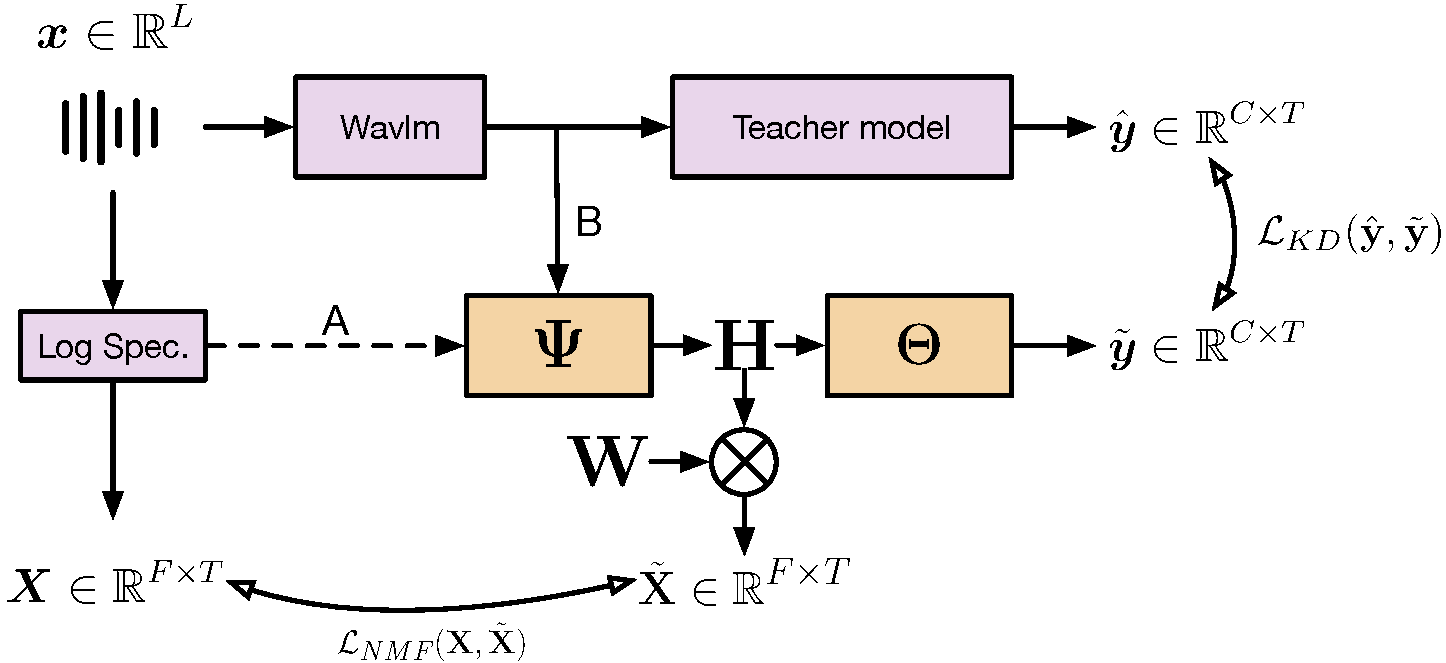
\includegraphics[width=\linewidth]{figs/nmf_model_icassp.pdf}
    \caption{Diagram of the proposed architecture for NMF-based multi-label segmentation explanation. The \textbf{A} and \textbf{B} branches represent the spectrogram and Wavlm-based proxy models respectively.}
    \label{fig:enter-label}
\end{figure}

\subsection{Multilabel segmentation formulation}

Acoustic segmentation is solved as a multilabel framewise classification task.
Let $\mathcal{S}=\{\mathbf{X}, \mathbf{y}\}$ be a training set composed of sequences of acoustic features $\mathbf{X}\in\mathbb{R}^{D\times T}$, where $D$ is the feature vector dimension and $T$ the number of frames, and the aligned annotations $\mathbf{y}\in \mathbb{R}^{C\times T}$, with $C$ being the number of classes. 
Let $f:\mathbb{R}^{D\times T} \rightarrow \mathbb{R}^{C\times T}$ be a parametric function that estimates the logits for each class from the sequence of features such as $\hat{\mathbf{y}}=f(\mathbf{X})$.
The parameters of $f$ are optimized to minimize a loss function $\mathcal{L}(\hat{\mathbf{y}},\mathbf{y})$, usually cross-entropy, with an iterative algorithm.

The sequence of feature $\mathbf{X}$ is extracted from the audio signal $\mathbf{x}\in\mathbb{R}^{L}$ by an additional function $\mathbf{X}=g(\mathbf{x})$. 
$L$ denotes the number of audio samples.

\subsection{Non-negative matrix factorization}

NMF has been extensively used for audio signal processing.
This approach factorizes a given non-negative matrix $\mathbf{X}\in\mathbb{R}^{F\times T}$ into two non-negative matrices: $\mathbf{W}\in\mathbb{R}^{F\times K}$, usually denoted as \textit{dictionary}, and $\mathbf{H}\in\mathbb{R}^{K\times T}$, denoted as \textit{activations}.
$K$ represents the rank of the factorization.
Both matrices are jointly learned by solving
\begin{equation}
    \mathbf{W},\mathbf{H} = \argmin_{\mathbf{W},\mathbf{H}} \|\mathbf{X}-\mathbf{W}\mathbf{H}\|_2^2,
\end{equation}
with a two-step optimization process \cite{lee2000algorithms}.
In this work, we consider the sparse NMF implementation \cite{le2015sparse} as suggested in \cite{parekh2023tackling}.
In our segmentation proxy model, the dictionary $\mathbf{W}$ is pre-learned while the activation $\mathbf{H}$ is extracted by a neural model and referred to as an embedding.
The proxy model architecture and the way NMF is integrated is described in the following subsection.

\subsection{Proxy model framework}

In this work, the $f$ model is pre-trained with frozen weights and serves as a teacher for the proxy model.
We use a similar approach as \cite{parekh2023tackling} where the proxy model is composed of two functions.
Let $\Psi$ be a function that maps a sequence of $F$-dimension feature vectors $\mathbf{S}\in \mathbb{R}^{F\times T}$ to the embedding $\mathbf{H}\in \mathbb{R}^{K \times T}$. 
The proxy model logits $\tilde{\mathbf{y}}\in\mathbb{R}^{C\times T}$ are obtained with an additional $\Theta$ function such as $\tilde{\mathbf{y}}=\Theta(\mathbf{H})$.
The spectrogram of the input audio signal $\tilde{\mathbf{X}}$ is also reconstructed from $\mathbf{H}$ with the pre-learned $\mathbf{W}$ dictionary:
\begin{equation}
    \tilde{\mathbf{X}} = \mathbf{W}\mathbf{H}.
\end{equation}

The training objective of such a model is composed of 3 loss terms.
The first trains the proxy model to mimic the teacher's decisions.
Considering multilabel segmentation, and following the common approaches in knowledge distillation \cite{}, we use the binary Kullback-Leiber (KL) divergence between the teacher and the proxy model output distributions:
\begin{equation}
\mathcal{L}_{KD}(\hat{\mathbf{y}},\tilde{\mathbf{y}})=\frac{1}{T}\sum_{t=1}^T\sum_{c=1}^C\hat{{y}}_{t,c} \log\Big(\frac{\hat{{y}}_{t,c}}{\tilde{{y}}_{t,c}}\Big) + (1-\hat{{y}}_{t,c}) \log\Big(\frac{1-\hat{{y}}_{t,c}}{1-\tilde{{y}}_{t,c}}\Big)
\end{equation}
where $c$ is the class index and $t$ the frame index.

The second loss term constrains the $\mathbf{H}$ embedding to minimize the NMF-based spectrogram reconstruction and is implemented as the squared l2-norm between the target spectrogram $\mathbf{X}$ and the reconstruction $\tilde{\mathbf{X}}$:
\begin{equation}
    \mathcal{L}_{NMF}(\mathbf{X},\tilde{\mathbf{X}})=\|\mathbf{X}-\mathbf{W}\mathbf{H}\|_2^2.
\end{equation}

The last loss term minimizes the l1-norm of the $\mathbf{H}$ embedding to enforce it to be sparse.
Having a sparse embedding reduces the number of active components, and makes the explanation step easier ().
Finally, the global training objective is the weighted sum of the 3 terms:
\begin{equation}
    \mathcal{L} = \alpha \mathcal{L}_{KD}(\hat{\mathbf{y}},\tilde{\mathbf{y}}) + \beta \mathcal{L}_{NMF}(\mathbf{X},\tilde{\mathbf{X}}) + \gamma \|\mathbf{H}\|_1,
\end{equation}
where $(\alpha, \beta, \gamma)$ is a triplet of hyperparameters to weight each term of the loss.



